\section{Programming in CUDA}

\paragraph{} By now, we have talked about the architecture of the GPU \footnote{Mainly about the Nvidia's architecture, but it 
can be quite well generalized to other GPU's.} by briefly discussing different notions - 
the execution model of threads and kinds of memory. Now, we will try to look at examples of CUDA codes and programs. 
We will try to refer to 
all these prior concepts to get a more detailed understanding. One may need to have a look at the section above 
to link the theory with the practice discussed here. I will do my best to choose the most illustrative examples (of those available 
in different resources) to explain specific concepts, 
as well as introduce some tools. 
Also, note that I use Linux. (\autoref{disclaimer}).

\subsection{Setup}
Before starting to write some code, we must install the necessary packages and libraries. Every computer and operating system 
has its own subtleties, so the best way to install necessary tools, one should check the documentation for the specific system
\footnote{See the installation methods and required components on \url{https://docs.nvidia.com/cuda/cuda-installation-guide-linux/index.html}.}.
For Linux, the main packages are \verb|CUDA| and \verb|CUDA-toolkits|. If we've already used our computer for some time,
we probably have Nvidia drivers installed. 



When we run a \verb|C| program, we need a compiler - arguably, the most common one \sout{and the best one} is \verb|gcc|. For \verb|C++|, 
we invoke his \textit{improved} version \verb|g++|. For CUDA programs, however, we need NVidia's CUDA compiler -
\verb|nvcc|. As we've discussed, the program 
consists of the host and device codes. The device code is just plain \verb|C|/\verb|C++| code, so \verb|nvcc| is also able 
to compile plain \verb|C|/\verb|C++|code. Note that the CUDA code has a \verb|.cu| extension.

\begin{listing}[!ht]
\begin{minted}[frame=single]{zsh}
   $nvcc -o main main.cu
   $./main
\end{minted}
\vspace{-0.7cm}
\caption{Compiling with nvcc and launching a CUDA program on Linux}
\label{nvcc_cuda}
\end{listing}

\vspace{-0.4cm}
If both of the programs do not return an error, the code has been compiled and launched successfully.

\subsubsection{Hello from CUDA}
Let's create our first CUDA and C++ program, and discuss every step below. 
\begin{minted}[frame=single, linenos=true]{cuda}
#include <stdio.h>   //for printf()
#define N_THREADS 4  //number of threads
#define N_BLOCKS 2   //number of block

__global__           //declaration specifier 
void hi_from_gpu(){  //kernel
    printf("Hi from GPU\n");
}
int main(){
    printf("Hi from CPU\n");
    hi_from_gpu<<<N_BLOCKS,N_THREADS>>>();   //invoking kernel
    cudaDeviceSynchronize();                 //synchronize CUDA program
    return 0;
}
\end{minted}

In the output of the following code, we \sout{should} get first \verb|Hi from CPU|, 
followed by 8 times \verb|Hi from GPU|. Let's discuss some aspects of the above code.
Line $5$ contains \verb|__global__| declaration specifier which tells 
the compiler that the following kernel (function) can be launched on the device.
In \verb|main()| function, on line 11, we call the kernel. This is the semantics to 
invoke a CUDA kernel. The \textit{arguments} in the angle brackets \verb|<<<,>>>| 
are the dimension of threads blocks respectively that the kernel will be run on\footnote{We will see further, some additional stuff can be passed
into these brackets, such as the size of memory and streams - concepts that will be seen in further sections
} \& . The type of these dimensions can be either an unsigned integer, or of the \verb|dim3| type, which we will mention in a moment. In this case, 
the GPU will call $2$ blocks, with $4$ threads each. This indeed results in 
$8 = 2\cdot 4$ invocations of \verb|printf()|. Finally, from the main function, we call 
the \verb|cudaDeviceSynchronize()| method, waits for all blocks before the main 
function returns.


\subsection{Threads \& blocks indexing}
Now let's dive in deeper, and access threads and block indexing by modifying our 
\verb|hi_from_gpu()| function:
\vspace{-0.5cm}
\begin{minted}[frame=single]{cuda}
#define N_THREADS 4
#define N_BLOCKS 2
__global__ 
void hi_from_gpu(){
    printf("Hi from GPU\n, from thread id %d and block id %d", 
    threadIdx.x, blockIdx.x);
}
\end{minted}
The output after executing from \verb|main|,
\vspace{-0.5cm}
\begin{minted}[frame=single]{zsh}
   $./main
   Hi from GPU, from thread id 0 and block id 0 
   Hi from GPU, from thread id 1 and block id 0 
   Hi from GPU, from thread id 2 and block id 0 
   Hi from GPU, from thread id 0 and block id 1 
   Hi from GPU, from thread id 1 and block id 1 
   Hi from GPU, from thread id 2 and block id 1 
\end{minted}
\vspace{-0.5cm}
We thus discovered how to access block's and thread's id's. The 
variables \verb|threadIdx| and \verb|blockIdx| are of type \verb|dim3|,
which is a simple structure, containing 3 unsigned int's. By accessing 
its \verb|.x| member variable, we are reffering to the 1D indexing. In general, 
threads are indexed using \verb|dim3| type. Thus, for a thread, living inside a block, there exist x, y and z 
dimensions. And same for the blocks, living in the grid - x, y and z components. 
Think of threads, 
We can launch many threads in many blocks, but how many? This depends on 
the hardware we are using.
To get these specifications, one can look up this information online or ask our computer.\footnote{
To do so, one must find where {\fontfamily{pcr}\selectfont cuda} is located. In my case, it is in 
{\fontfamily{pcr}\selectfont /opt/cuda/}.
Once here, we seek for {\fontfamily{pcr}\selectfont /samples/1\_Utilities/deviceQuery/} 
(or something similar). 
From here, we execute {\fontfamily{pcr}\selectfont ./deviceQuery}.   
}.
Alternatively, we can perform this in code. The device properties can be stored in a structure. In the 
CUDA API, this structure is called \verb|struct cudaDeviceProp|, which has many attributes in it. A few of them are \verb|int clockRate|, \verb|int maxGridSize|, \verb|size_t totalGlobalMem| and many more ((see the official documentation). 
To actually get the properties, one passes the initialized struct's pointer to the function: 
\verb|cudaGetDeviceProperties(&dev_props)|. After the invocation of this function, we should 
be able to get the properties by setting \verb|dev_props.maxGridSize| for example.

\subsection{Memory}

\subsubsection{Vector addition}
The first \textit{useful} example 
that is usually introduced in CUDA tutorials is the vector addition. This exaple
perfectly illustrates the need of GPU parallel model. Indeed, the component of the resulting
 vector $x$ $x_i$ does not depend on other components. So the formula for vector addition is given by 
 $x_i = a_i + b_i$. In sequential execution, we would create a loop, iterate over all elements and 
do something like \verb|x[i] = a[i] + b[i]|. In order to parallelize this workflow, we must initiate $N$ 
threads, with $N = \text{number of components in the vector}$. In \verb|C++|, which simply runs on the host, we create the threads 
using the standart \verb|std::thread|. We know, however, that the CPU does not have many threads (probably from 4 to 12 in most cases). 
This is where the GPU with its multithreaded architecture comes in. The idea here is to launch $N$ threads which are spread over many blocks.
\newline 
To discover memory allocation with code examples, we will consider vector addition. And to do that, 
one must first cover thread \& block indexing for a more general case.

\paragraph{A more complex indexing.} 
We know that the number of threads in one 
block is limited. Let's check on Nvidia's official CUDA documentation \cite{center} concerning threads indexing. 
\begin{quote}
   \textsl{For convenience, {\fontfamily{pcr}\selectfont threadIdx} is a 3-component vector, 
   so that threads can be identified using a one-dimensional, 
   two-dimensional, or three-dimensional thread index, forming a one-dimensional, two-dimensional, 
   or three-dimensional block of threads, called a thread block. This provides a natural way to invoke computation across 
   the elements in a domain such as a vector, matrix, or volume.
   The index of a thread and its thread ID relate to each other 
   in a straightforward way: For a one-dimensional block, they are the same; for 
   a two-dimensional block of size $(Dx, Dy)$,the thread ID of a thread 
   of index $(x, y)$ is $(x + y\cdot Dx)$; for a three-dimensional block of size $(Dx, Dy, Dz)$, the thread ID of a 
   thread of index $(x, y, z)$ is $(x + y\cdot Dx + z\cdot Dx\cdot Dy)$.}
\end{quote}

Before writing some code, let's try to visualize the Nvidia's quote.
\begin{figure}[H]
   \centering
   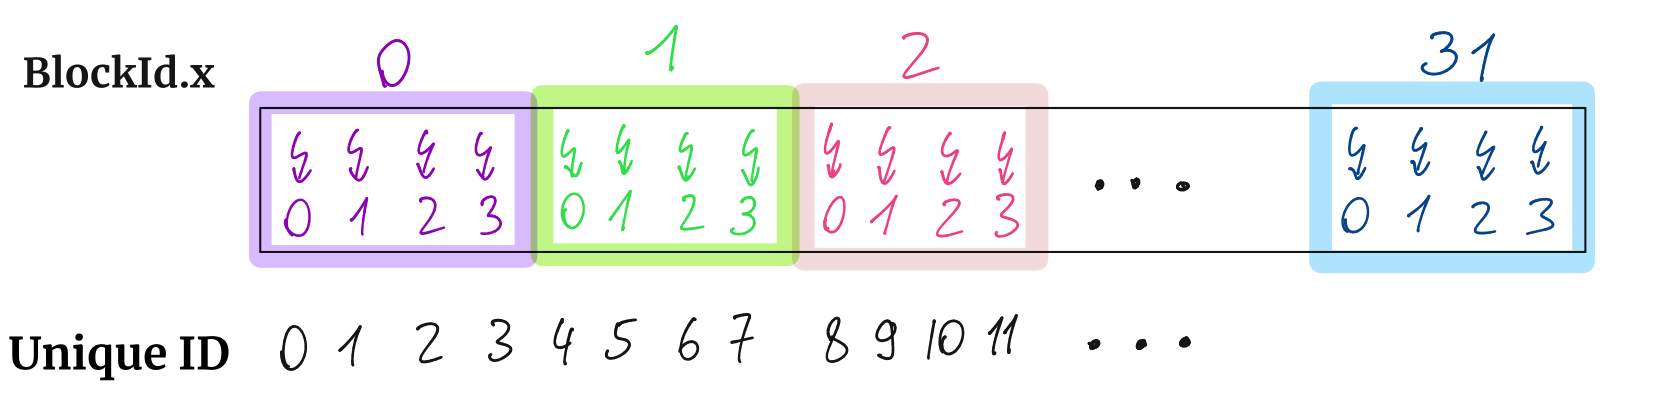
\includegraphics[scale=0.25]{pngs/tindexing.png}
   \caption{Simple example to illustrate a plain 1D indexing (supposing a block 
   contains 4 threads). We see how the expression \textsc{blockIdx.x*blockDim.x+threadIdx.x} is used (see below). 
   One can easily extrapolate the indexing to 2D and 3D cases, as described in the Nvidia documentation above.
   }
   \label{fig:tindexing}
\end{figure}
Let's now write code to add two vectors, using a 2D indexing \footnote{This is the first and almost the only \textbf{full} example of a cuda program. 
That is, the author will mostly provide the key aspects of the newly introduced features, thus skipping the usual parts of defining things, of allocating 
memory, freeing it, etc.}: 

\begin{listing}
\begin{minted}[
   frame=single,
   framesep=2mm,
   baselinestretch=0.8,
   fontsize=\footnotesize,
   linenos 
   ]{cuda}
#include "stdio.h"
#define N_THREADS 512
#define N_BLOCKS 64 
void init_host_vector(double *a, double *b);
void check_result(double *res);

__global__ 
void add_vec(double *a, double *b, double *res){
    //compute the index
    int id = blockIdx.x*blockDim.x+threadIdx.x;
    if(id < N_THREADS*N_BLOCKS){
        res[id] = a[id] + b[id];
    }
}

int main(){
    const int size_in_bytes =N_THREADS*N_BLOCKS*sizeof(double);
    //initialize the data on HOST
    //malloc() (C) or new (C++) 
    double *hst_a = (double *)malloc(size_in_bytes);
    double *hst_b = (double *)malloc(size_in_bytes);
    double *hst_res = (double *)malloc(size_in_bytes);

    init_host_vector(hst_a, hst_b);

    //allocate memory on GPU
    double* dv_a;    cudaMalloc(&dv_a, size_in_bytes);
    double* dv_b;    cudaMalloc(&dv_b, size_in_bytes);
    double* dv_res;  cudaMalloc(&dv_res, size_in_bytes);

    cudaMemcpy(dv_a, hst_a, size_in_bytes, cudaMemcpyHostToDevice);
    cudaMemcpy(dv_b, hst_b, size_in_bytes, cudaMemcpyHostToDevice);

    add_vec<<<N_BLOCKS, N_THREADS>>>(dv_a, dv_b, dv_res);
    cudaDeviceSynchronize();
    cudaMemcpy( hst_res, dv_res, size_in_bytes, cudaMemcpyDeviceToHost );

    check_result(hst_res);

    cudaFree(dv_res);   free(hst_res);
    cudaFree(dv_a);     free(hst_a);  
    cudaFree(dv_b);     free(hst_b);
    return 0;
}
\end{minted}
    \caption{Basic vector addition, using sequential thread indexing. \cite{tuomanen2018hands}}
\end{listing}

Ok, there are multiple aspects to discuss...

First let's discuss the code. First on the device. Remember we discussed the global GPU memory. 
The line 31 we're working with memory. The classical pipeline of any CUDA program
execution, is usually the following:

\begin{enumerate}
\setlength\itemsep{-0.5em}
   \item Begin code on host.
   \item Allocate memory on host.
   \item Allocate memory on device.
   \item Calculations performed on the device.
   \item Host treats the data.
   \item main() gets returned.
\end{enumerate} 

\paragraph{Allocate memory on host.} To allocate memory on the host, 
we proceed with the usual C \verb|malloc()| function and naturally 
casting the returned pointer to \verb|double*| (don't forget 
to free memory at the end by \verb|free()| function). 
Then we call a simple function \verb|init_host_vector()| that will just initialize the data 
to some values, let's say to simple $0,1,2,3, ...$. 
\paragraph{Allocate memory on device.} Then we allocate \textbf{global memory} on the GPU, 
by calling the \verb|cudaMalloc()| function. Note the arguments that this function takes - 
a \textbf{pointer to pointer} - \verb|(<type> **)| and the size in bytes. 

 
\paragraph{Data copying} between the host and the device is done using the \verb|cudaMemcpy()| function. Also, pay attention 
to the parameters - 
\verb|cudaMemcpy(void* destination, void* source, size_t size_in_bytes,| \newline \verb|enum cudaMemcpyKind kind)|,
with \verb|kind| \footnote{Here, I described the parameters in details. However, further on,
the author will not be that precise. The reference for this function was taken from 
\url{http://horacio9573.no-ip.org/cuda/group__CUDART__MEMORY_g48efa06b81cc031b2aa6fdc2e9930741.html}. 
For further function descriptions, always have a look at it.}
specifying how to copy. In code, it is understandable that the destination is the 
device and the source is the host.

\vspace{-0.8cm}
\paragraph{Calculation.} The kernel computes the sum of a vector of size $512\cdot 64 = 32768$. 
Therefore $64$ blocks of $512$ threads are launched, and $32768$ threads independently execute the \verb|add_vec()|
function. In the kernel, a unique ID is assigned to the thread(line 10) (see the indexing \textit{policy}  see \ref{fig:tindexing}). 
The ID's span from $0$ to $32768$, without ever repeating themselves and covering all the numbers in the interval.
We also add a simple \verb|if()| statement, to be sure, that the thread's ID does not exceed the size of the vector.
Thus every thread does exactly one calculation \footnote{Of course, without taking into account the calculation of the id.}.
Remember that the memory, in which these processes are happening, is the global memory. 

\vspace{-0.8cm}
\paragraph{Terminating.} After the kernel, we call the usual synchronization function, which will, as usual, wait for all the threads and blocks 
to finish the calculations. 
Then, a simple check function on the host, simply to ensure, that the parallel vector addition was successful and that we've received the correct result.
And finally, the \verb|cudaFree()| method, does exactly what is expected - 
frees the allocated memory on the GPU, the exact same things, as the \verb|free()| does in a usual \verb|C| code.

Let's also try to link this piece of code to the section about warps. Remember, 
threads are scheduled by the SM into warps - groups of 32 threads (\autoref{warps}). 
In this case, we're launching a total of $\nicefrac{512}{32} = 16 \text{warps}$ for each 
block, and 64 independent blocks. While working with CUDA threads, it is advised to work with 
the number, which is a multiple of $32$ (the thing we've done in this example). Indeed, imagine, if we were to launch $513$ threads on a block.
Then the SM would schedule 17 warps. This number of warps is the same as if we would launch $544$ threads in a block.
Indeed, this will launch $16\cdot 32 = 512$ threads (executed simultaneously in one warp) \textbf{and} 
one additional thread on an almost empty/unoccupied warp. 

One could also be interested in the difference in the execution time between 2 different
 configurations - either $64\text{threads}\cdot 512\text{blocks}$ or $32\text{threads}\cdot 1024\text{blocks}$
 The benchmarking is very important and useful in GPGPU programming. Different tools and techniques for  
 benchmarking CUDA programs will be discussed in further sections.

\subsubsection{Multiple dimension memory}
By now, we've looked into the global one-dimensional 
memory allocation (and copying) on device. Suppose you would like to work 
with 2D allocated memory. It is clear that we could work without the ability to explicitly allocate 2D or 3D arrays. 
Indeed, if we want to work with, let's say, a 2D matrix, we could simply 
transform it into a 1D vector of size rows$\cdot$cols.
However, there is a feature in the CUDA API, that lets us to allocate 2D, and even 
3D memory \cite{MemoryAlignment}. 
The method that implements 2D memory allocation is \verb|cudaMallocPitch| with the following signature:


\begin{minipage}[h]{0.5\textwidth}
   \vspace{-1cm}
     \begin{minted}[frame=single,framesep=2mm]{cuda}
cudaMallocPitch( void** devicePtr,
                size_t* pitch,
                size_t widthInBytes,
                size_t height);
     \end{minted}
     \captionof*{figure}{The signature of function. Some new terminology 
     given on the \hyperref[fig:pitch]{right}.}
\end{minipage}
\begin{minipage}{0.4\textwidth}
   \hspace{0.2cm}
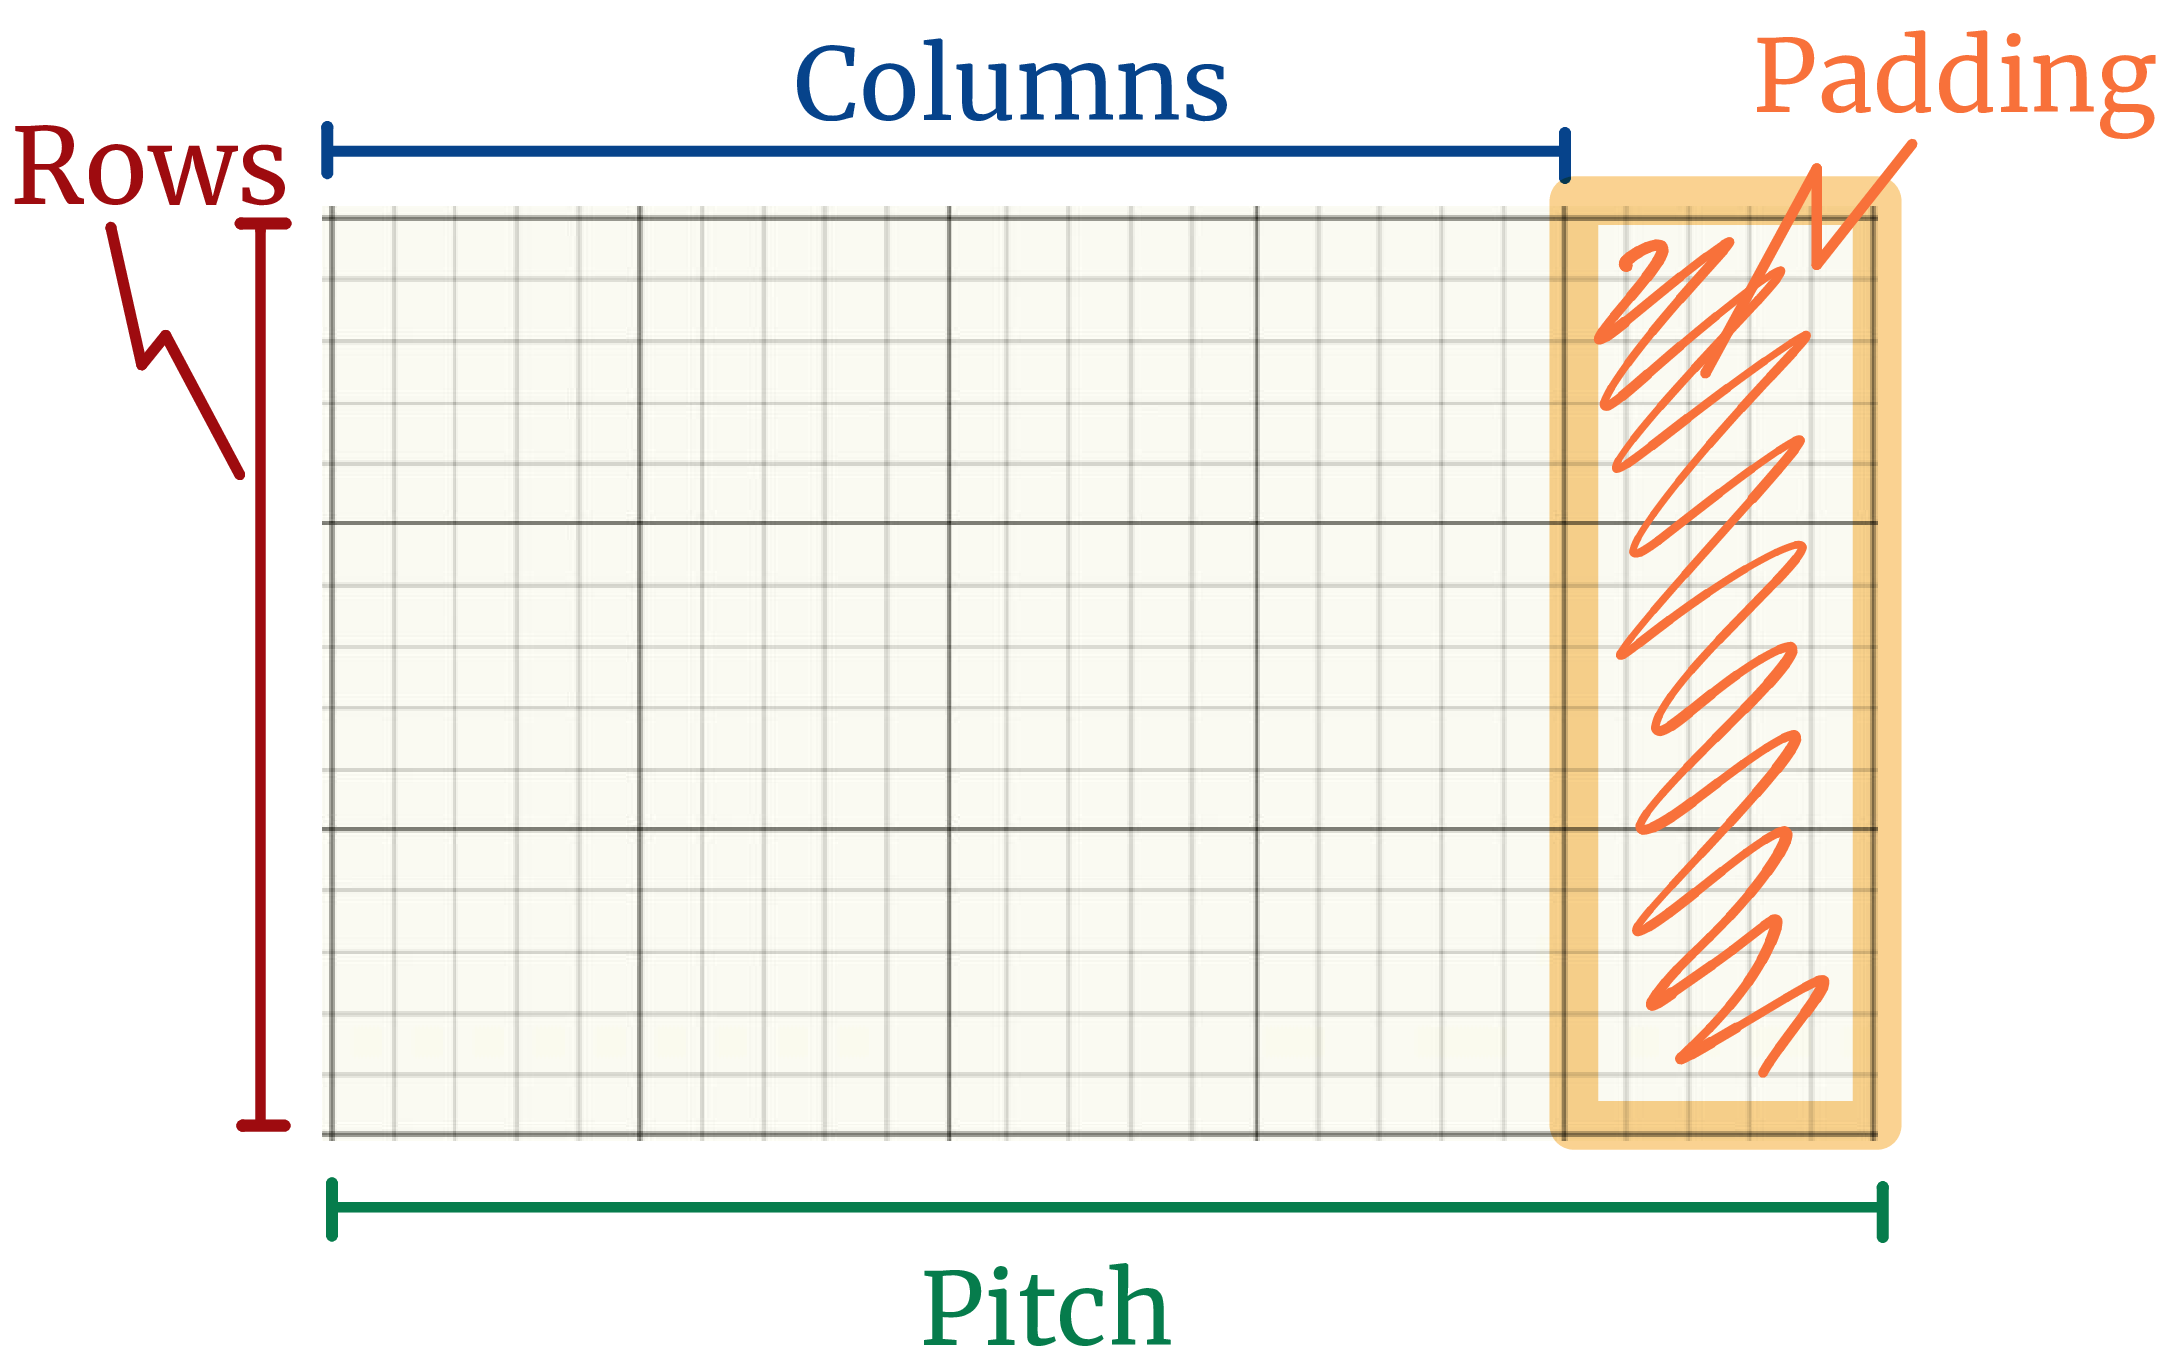
\includegraphics[scale=0.10]{pngs/pitch.png}
\label{fig:pitch}
\hspace{1cm}
\end{minipage}

This function is allocating \textbf{at least} width$\times$height bytes array
As we have seen, the allocation on the device is followed by the data copy from 
the host. There is also a special function to do so - \verb|cudaMemcpy2D()|. Apart from allocating 
and initializing the device data, we should be able to access it. So let's consider a code snippet
that does so:

\begin{listing}[!ht]
\begin{minted}[frame=single, framesep=1mm]{cuda}
int main(){
   float *A, *dA;
   size_t pitch;
     
   A = (float *)malloc(sizeof(float)*N*N); // allocate on host
   cudaMallocPitch(&dA, &pitch, sizeof(float)*N, N); // allocate on device

   //copy memory
   cudaMemcpy2D(dA,pitch,A,sizeof(float)*N,sizeof(float)*N, N,\
      cudaMemcpyHostToDevice);
         /*...*/
}
__global__ void access_2d(float* devPtr, size_t pitch,\
            int width, int height) {
    for (int r = 0; r < height; ++r) {
        float* row = (float*)((char*)devPtr + r * pitch);
        for (int c = 0; c < width; ++c) {
            float element = row[c];
        }
    }
}
\end{minted}
\caption{To get this straight, one should know 2D array work in pure C. 
  Indeed, to access an element, we first identify the current row, by doing some pointer manipulations. 
  And then, once the pointer to the very beginning of the row is identified, we iterate over this 
  row, by accessing it sequentially. Also note that in the code, in order to identify the 
  row for the next iteration (i.e. it's $0$'s element pointer), one uses the size of the pitch, and 
  not of the width. We see that this 2D pitch is allocated 
    \textbf{automatically} by the CUDA memory management system \cite{blog_2020}
  }
\label{allocation2d}
\end{listing}


As you might have guessed, this memory access is not extremely efficient. As one may say, \textsc{this is for educational purposes only}. In the documentation, it is recommended 
to use these functions to allocate and initialize the 2D memory on device. Hopefully, we all can find 
use cases of this memory and efficient indexing \footnote{There are a lot more of memory allocation, \& memory copy methods, 
provided in the CUDA API. For example {\fontfamily{pcr}\selectfont cudaMallocArray()}, which has also a different signature.
The different methods, dedicated to memory allocation and management can be observed \url{https://courses.cs.duke.edu/cps296.3/fall09/cuda_docs/html/group__CUDART__MEMORY_ge56101fe6f1ce0b48f163632f6862ae4.html#ge56101fe6f1ce0b48f163632f6862ae4} }.

\subsection{More on Memory}
\subsubsection{Shared memory vs global memory}

For now, in the examples, we've only looked into the global (\& pinned) memory. It is global and accessible 
for all threads in all blocks for both read and write operations, and yet having high latency, compared to 
more local memory types, such as the shared one. Shared memory's scope is one \underline{thread block}. Thus, if, let's say,
a block contains 16 threads, the shared memory can only be read and modified by 16 local threads. If one wants to operate on it 
locally, the data must be copied to it. Therefore, if one wants this memory to be accessed/modified by 2 thread blocks ($=32$ threads), one 
must make sure that the data has been copied to the shared memory of the two blocks.

Let's now consider a more complex and yet classical example - matrices. Recall basic matrix operation - 
\begin{itemize}
   \setlength\itemsep{-0.5em}
   \item If $A$ - $m\times n$ matrix ($m$ rows and $n$ columns), it can be added to some 
   other matrix $B$ of same size $m\times n$, by adding element-wise each element $a_{i,j}+b_{i,j}$. 
   \item One can multiply two matrix $A$ and $B$ - $C = A\cdot B$ by using the formula 
   $c_{i,j} = a_{i,1}\cdot b_{1,j} + a_{i,2}\cdot b_{2,j} + ... + a_{i, n}\cdot b_{j,n}$, only if the matrix 
   $A$ is of size $m\times n$ and $B$ of size $n\times p$. In short, the resulting 
   element $c_{i,j} = \sum_{k=1}^{k=n}a_{i,k}\cdot b_{k,j}$ and yields $C$ of size $m\times p$.
\end{itemize}

One can perform these operations using the global memory, or shared memory.

\paragraph{Global} version code snippet is given down below.


\begin{listing}
\inputminted[linenos=true, frame=single]{cuda}{cucodes/matmulglob.cu}
    \caption{Basic, yet important, global memory usage. \cite{tuomanen2018hands}}
\end{listing}

Before moving to the code discussion, let's make a small \textit{intermezzo}
on transforming 2D array to 1D, to make things clear and easier for further analysis:

\noindent\fbox{
   \parbox{0.96\textwidth}{
   Suppose we are given a 2D array (matrix). But we know that, behind the scenes,
   (even if we're accessing a[i][j] in many programming languages), it all breaks 
   down to contiguous, linear memory addresses. So suppose you have allocated 
   a 1D array arr of size $N$. The, you could access your i'th element by doing {\fontfamily{pcr}\selectfont arr[i]}  
   (supposing C or C++) or by doing {\fontfamily{pcr}\selectfont*(arr + i)}, where 
   {\fontfamily{pcr}\selectfont arr} - the address of the 0'th element 
   of the array . So the formula is given by $\text{A}_{i^{th}} = A_{0} + \text{sizeof(type)}\cdot i$, where 
   $A_0$ - the first (0'th) memory address and sizeof-the size of one memory field (e.g. sizeof(char) = 1).
   Suppose now, that we've allocated a 2D memory array of size $M\text{rows }\times N\text{cols}$. For the first row
   one can apply our previous formula - $A_{0,j} = A_{0} + \text{SZ}\cdot j$. However, if $j$ is 
   greater than $N$ - the number of columns, a problem occurs. If we work in 2D indexing, over a loop, we would just 
   \textit{reset} our index $j$ to 0 and increment $i$ (if $j=N-1$). However, in a flattened 2D case, in order to 
   access $A_{i,j}$ address-wise, we use the expression 
   $A_{i,j} = A_{0} + \text{sizeof(type)}\cdot N\cdot i + j)$. One can easily check, that this expression is consistent with all the 
   examples. This expression is for row-major arrays - accessing successive elements in a certain row.
   }
   \label{intermezzo1d2d}
}
\vspace{1cm}


Okay, now we can attack the code. From line 13 to 21, we are initializing the data and 
allocating memory. The lines 27 \& 28 are initializing the dimensions 
(number of threads in x,y directions and the number of blocks in the x, y directions), that the kernel will be launched on. 
Note that we are using 2D indexing for the first time.
In this case, \verb|grid_dim| is the dimension of the grid, 
in which blocks are contained. The \verb|block_dim| is the block dimension - the number of threads in the block. 
In this case there are $16\cdot 16 = 256\text{threads}$ and $\frac{32}{16}\cdot \frac{32}{16} = 2\cdot 2 = 4 \text{blocks}$. 
So there are $256\cdot 4 = 1024 \text{threads}$ partitioned between 4 blocks. This is exactly what we need, 
because the resulting matrix $C$ is exactly $32\times 32$, which gives us 1024 elements. Therefore, if everything goes well,
each thread will perform the calculation for each element $c_{i,j}$ of the matrix $C$. 
In theory, we would like that 
each thread iterates over one line of the matrix $A$ and one column of $B$. Remember the \hyperref[intermezzo1d2d]{1D to 2D mapping}. 
is going through all the elements in the row $i$ of the matrix $A$ (line 43). 



\vspace{-0.9cm}
\begin{gather*}
 A_{i, h} = A_{0} + i\cdot N_{cols(A)} + h
\\
B_{h,j} = B_{0} + h \cdot N_{cols(B)} + j
\end{gather*}
These equations (at least the first one) are exactly predicted by \hyperref[intermezzo1d2d]{1D to 2D mapping} and
are represented on the lines 43 and 44 of the code snipped. 
Finally, once each thread runs over its own row and column, it is 
gathering the result by assigning this accumulated sum to the 
\verb|C[i][j] = C[i*Width + j]|, where i,j - row id's and column id's respectively\footnote{This 
aspect is not simple yet basic. This is a common CUDA pattern, which needs to be understood correctly 
\sout{(or at least know where to look for)}. So one should try to visualize the indexing process and the algorithm workflow. }


\paragraph*{Shared memory} is one of the key, to control the efficiency of a CUDA program. 
As we've mentioned several times before, the shared memory is only visible in the block's scope. That means that 
if, we would want to make the shared memory visible \& accessible to all threads in the entire kernel, we would 
need to allocate (and transfer the data to) shared memory, which belongs to independent blocks. 
Remember the analogy of the \hyperref[grocery_store]{grocery store}.
It's up to the programmer to decide, whether it would be reasonable to spend time on algorithm design, using shared memory, and its allocation
 (which, of course, takes time, but has little latency, when using it), or to high-latency global memory access.
So let's have a look at a shared memory code snippet\footnote{For space-saving's sake, only a snipped is provided. The skipped pieces are usual steps of 
memory allocation, freeing resources, etc...}.
demonstrating shared memory usage for matrix multiplication. 
Let's first discuss the general strategy. As we have said, the shared memory is much smaller in terms of size 
than the global one. So here, the main idea is to divide the \textit{big} matrices $A$ and $B$, that we're multiplying into smaller
sub-matrices, which will be loaded into the shared memory later of each independent block.

\begin{figure}[ht!]
   \centering
   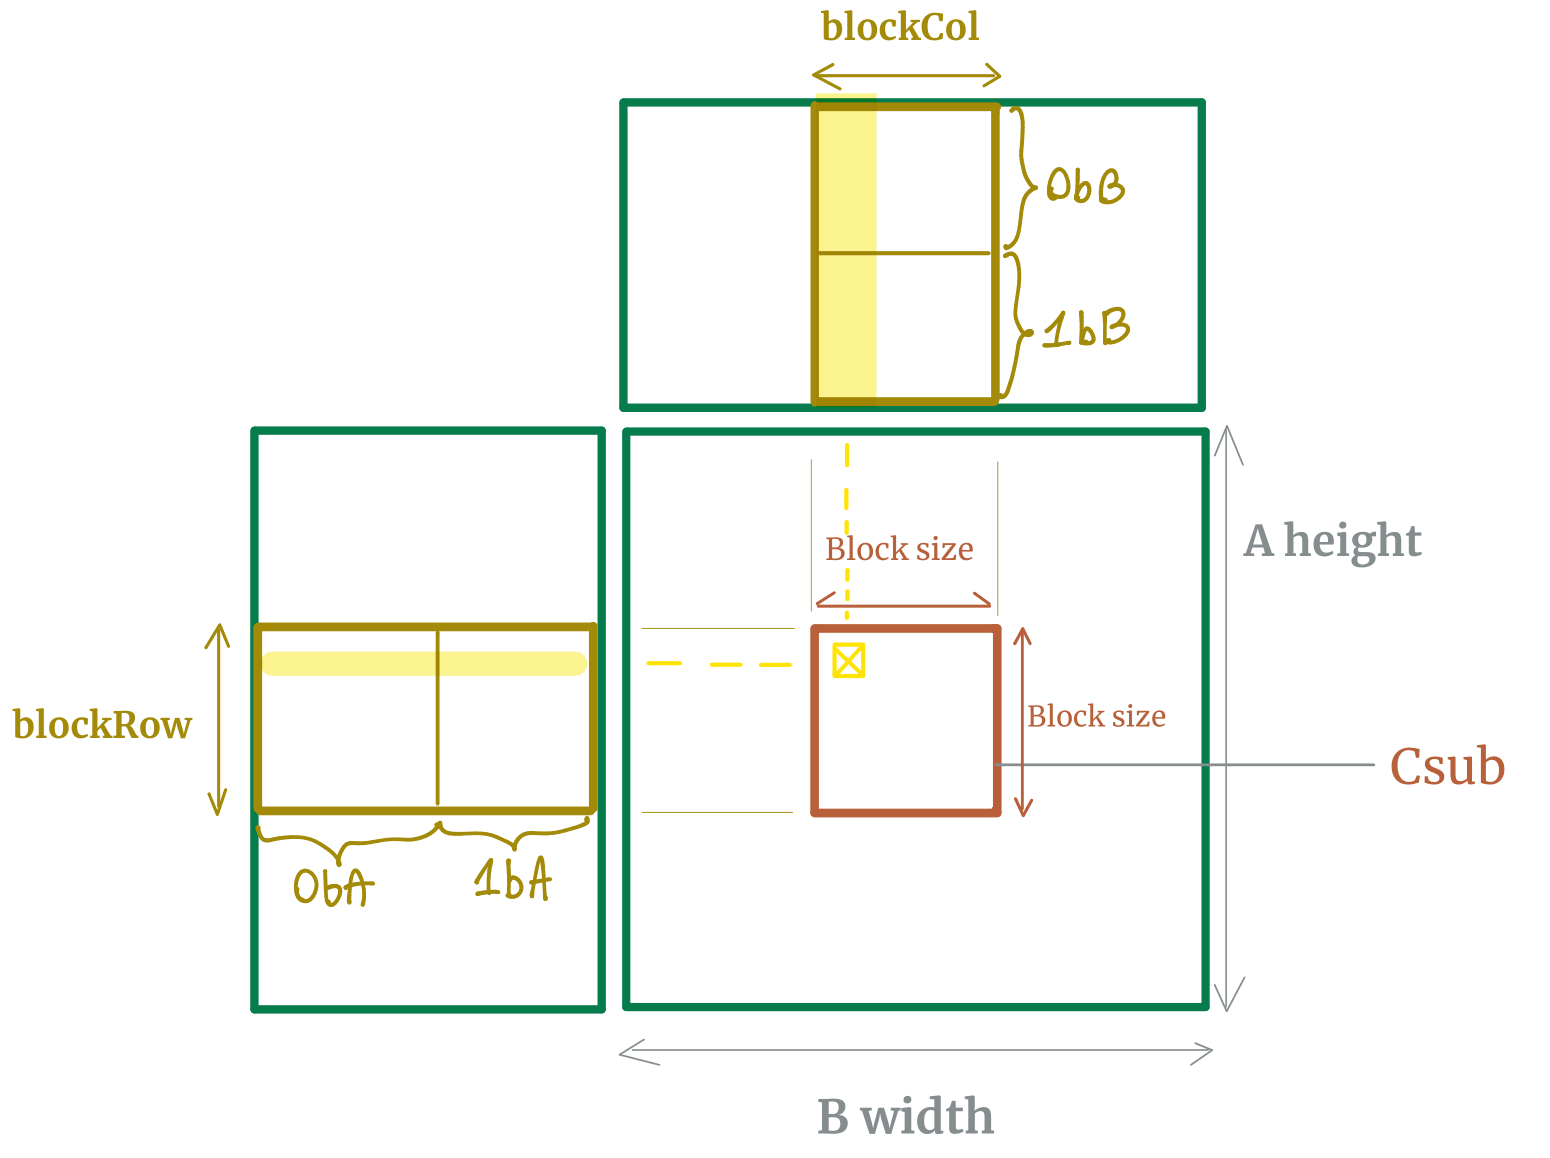
\includegraphics[width=0.6\textwidth]{pngs/globalmatrix.png}
   \vspace{-0.5cm}
   \caption{Scheme of 2D matrix multiplication, using Shared memory}
   \label{global2d}
\end{figure}


Let's look at the code describing this strategy:

\begin{minted}[frame=single, framesep=1mm, linenos=true]{cuda}
typedef struct{
   int width; int height; int stride;
   float *elements;
}Matrix;

__device__ float GetElement(const Matrix D, int row, int col)
{
    return D.elements[row * D.stride + col];
}

__device__ Matrix GetSubMatrix(Matrix D, int row, int col) 
{
    Matrix sub;
    sub.width    = BLOCK_SIZE;
    sub.height   = BLOCK_SIZE;
    sub.stride   = D.stride;
    sub.elements = &D.elements[D.stride * BLOCK_SIZE * row
                                         + BLOCK_SIZE * col];
    return sub;
}

 __global__ void mult_global(Matrix A, Matrix B, Matrix C)
{
    // blockRow & blockCol (see image)
    int blockRow = blockIdx.y;
    int blockCol = blockIdx.x;

    // Create Csub, initial matrix
    Matrix Csub;
    Csub = GetSubMatrix(C, blockRow, blockCol);
    float Cvalue = 0; //we will accumulate values (see figure above)

    // Thread row and column within Csub
    int row = threadIdx.y;
    int col = threadIdx.x;

    // Loop over all the sub-matrices of A and B 
    // Multiply each pair of sub-matrices together
    for (int m = 0; m < (A.width / BLOCK_SIZE); ++m) {//iterate over 
                                          //sub-matrices//of A(see fig above)  
        Matrix Asub=GetSubMatrix(A, blockRow, m);//Asub of A(m-the index of row)
        Matrix Bsub=GetSubMatrix(B, m, blockCol);//Bsub of B(m-the index of col)

        // shared memory to store Asub and Bsub
        __shared__ float Asub[BLOCK_SIZE][BLOCK_SIZE];
        __shared__ float Bsub[BLOCK_SIZE][BLOCK_SIZE];

        // Each thread loads one element of each sub-matrix Asub and Bsub
        As[row][col] = GetElement(Asub, row, col);
        Bs[row][col] = GetElement(Bsub, row, col);

        //All threads must be synced, to be sure all data is loaded properly
        __syncthreads();

        // Use matrix multiplication formula to get the Csub element
        for (int e = 0; e < BLOCK_SIZE; ++e){
            Cvalue += Asub[row][e] * Bsub[e][col];
        }

        __syncthreads(); //synchronize before new sub-matrices are loaded
    }
    C.elements[row * A.stride + col] = Cvalue;
}
   int main(){
      /*init matrices on host
      * init matrices on device with cudaMalloc(),
      * copy data from host to device
      */
   dim3 dimBlock(BLOCK_SIZE, BLOCK_SIZE);
   dim3 dimGrid(B.width / dimBlock.x, A.height / dimBlock.y);
   mult_global<<<dimGrid, dimBlock>>>(d_A, d_B, d_C);
   }
\end{minted}

Okey, let's now discuss in detail the execution of the kernel \verb||, and try to make as more analogy as possible
with the scheme above.
\begin{enumerate}
   \item The matrices are assumed to be multiples of BLOCK\_SIZE (block dimension in fact). In this case, let's say $32\times 32$. So, 
   from the main function, we're launching 32 threads in each block, and $2\times 2 = 4$ blocks in a grid. Thus we have 
   $32\times 32\times 4=4096 \text{ threads}$, organized in a grid of 4 blocks. So there is a kind of mapping between 
   the 2D matrix and the threads partitioned into blocks.
   Keep that launched chunk of threads in mind. 
   \item The first thing we do in the kernel is attribute the block row and column ids. They correspond to blockRow and blockCol, 
   annotated in the figure \ref{global2d}. There will thus be 4 sub-matrices to which, to which each block will be assigned to (as we've said 
   that the block is of size $16\times 16$ and the matrix size is $32\times 32$). Remember that
   the shared memory is \textbf{only visible inside a block}. Thus the possible configurations of the indices are given by 
   $(A_{row}=0, B_{col}=0)$, $(A_{row}=0, B_{col}=1)$, $(A_{row}=1, B_{col}=0)$ and $(A_{row}=1, B_{col}=1)$. These indices correspond to the 
   \textit{olive color} strips on the figure, labeled with BlockRow and BlockCol respectively.
   \item Then we're initializing the sub-matrix $C_{sub}$ - its dimensions, elements and stride.
    The stride, in our case, is the offset we need to take into account when computing the elements in the row-major form. Note that it is not always
    the same as matrix width. For example, when we're dealing with the submatrix, the stride does not equal to its width, but rather 
    \textbf{the original matrix width}. Indeed, the size of the submatrix does not affect the element's addresses in memory.
    This sub-matrix $C_{sub}$ is illustrated in figure \ref{global2d}. 


        This gives us the ability to keep 
   track of the sub-matrix within each block. Remember, the multiplication 
   of (sub-)matrices involves the accumulation of element-wise multiplication, so we're initializing the temporary sum to $0$.
   \item The initialization is followed by the initialization of sub ids. These are the thread ids \textbf{within a block}.
   Thus these id's will be uniquely identified for each thread within the block, launched on a unique kernel instance. And, as we know, each block will be responsible 
   for one sub-matrix of $C$ - $C_{sub}$. These ids are represented by yellow rows and columns on figure.
   \item Now, an important assumption will be made - the number of blocks contained in A's matrix width is the same as the number of 
   blocks contained in the B's matrix height\footnote{This is an assumption, that is, as we say W.L.O.G - without loss of generality. 
   Indeed, if this assumption is not the case, one could modify a bit the code for it to work without this assupmtion.
   However, this is neither a problem, because, one can allocate and perform operations on a bit bigger matrices, without big issues in 
   performance}. This is the reason why we can use the first loop, to iterate over A'th width and B'th height \textit{simultaneously}. 
   \item As mentioned just above, we can simultaneously iterate over A'th width and B'th height, thus simultaneously obtaining the sub-matrices 
   $A_{sub}$ and $B_{sub}$. After getting the sub-matrices $A_{sub}$ and $B_{sub}$, we allocate shared memory \verb|As| and \verb|Bs| for 
   $A_{sub}$ and $B_{sub}$ using the \verb|__shared__| directive. Note here, that each thread in the block is retrieving \textbf{one, and only one element} of the matrix. 
   Indeed, the \verb|getElement()| method retrieves only one element from global to local memory. This is the most important step in this 2D matrix multiplication.
   \item After each thread retrieves the data \textbf{within the block}, we would like all threads to be done with synchronization. Indeed, in global memory's case, 
   each thread accesses the global memory independently, with a unique ID. Here, with the shared memory, we introduce a kind of independence between threads, by making them all access to the same block-local shared memory, by 
   making them all retrieve local data. So, for example, suppose we have a $4\times 4$ sub-matrix. Each thread within the block loads one element into shared memory (seen by the other 15 threads). So before 
   making the calculations, we want all the 16 data to be loaded into shared memory.
   \item Afterwards, we are finally doing calculations on the sub-matrix, using the previously retrieved elements of $A_{sub}$ and $B_{sub}$ into \verb|As| and \verb|Bs| respectively.
   Remember here that \verb|row| and \verb|col| are unique for each thread. Once again - This step is illustrated in the figure: the iteration is performed through the yellow 
   line's multiplication element-wise. And the \textbf{unique} elements, attributed to the threads are the \verb|row| and \verb|col| indices. This is the final result 
   we want to achieve: \textit{each thread within the block multiplies the \textbf{row} of $A_{sub}$ and the \textbf{col} of $B_{sub}$ element-wise, to get only one element of the $C_{sub}$ sub-matrix}.
   \item The final step of the kernel is to copy each element of the $C_{sub}$ sub-matrix to the global memory. Once again, 
   as each thread is doing its own $Csub_{i,j}$ element, it is just copying only \textbf{one} element to global memory.   
\end{enumerate}
   Note that apart of the \verb|__shared__| directive, other, new technical aspects were used. First - the \verb|__device__| directive.
   It declares a function, which can \textbf{only} be called from the device function (the one declared with \verb|__global__|). These device functions 
   can return different types. Second - the shared memory with the \verb|__shared__| directive. As discussed above, this is shared memory, only seen within the block.
    

   As mentioned, this is a very fundamental example, yet not simple, and takes time to understand. The reader \sout{and the author} must go through the code 
   and the illustration several times. As well as going through multiple particular instances of the code, with particular instances of the block and threads ids.


\begin{figure}[h!]
   \centering
   \subfloat[\centering]{{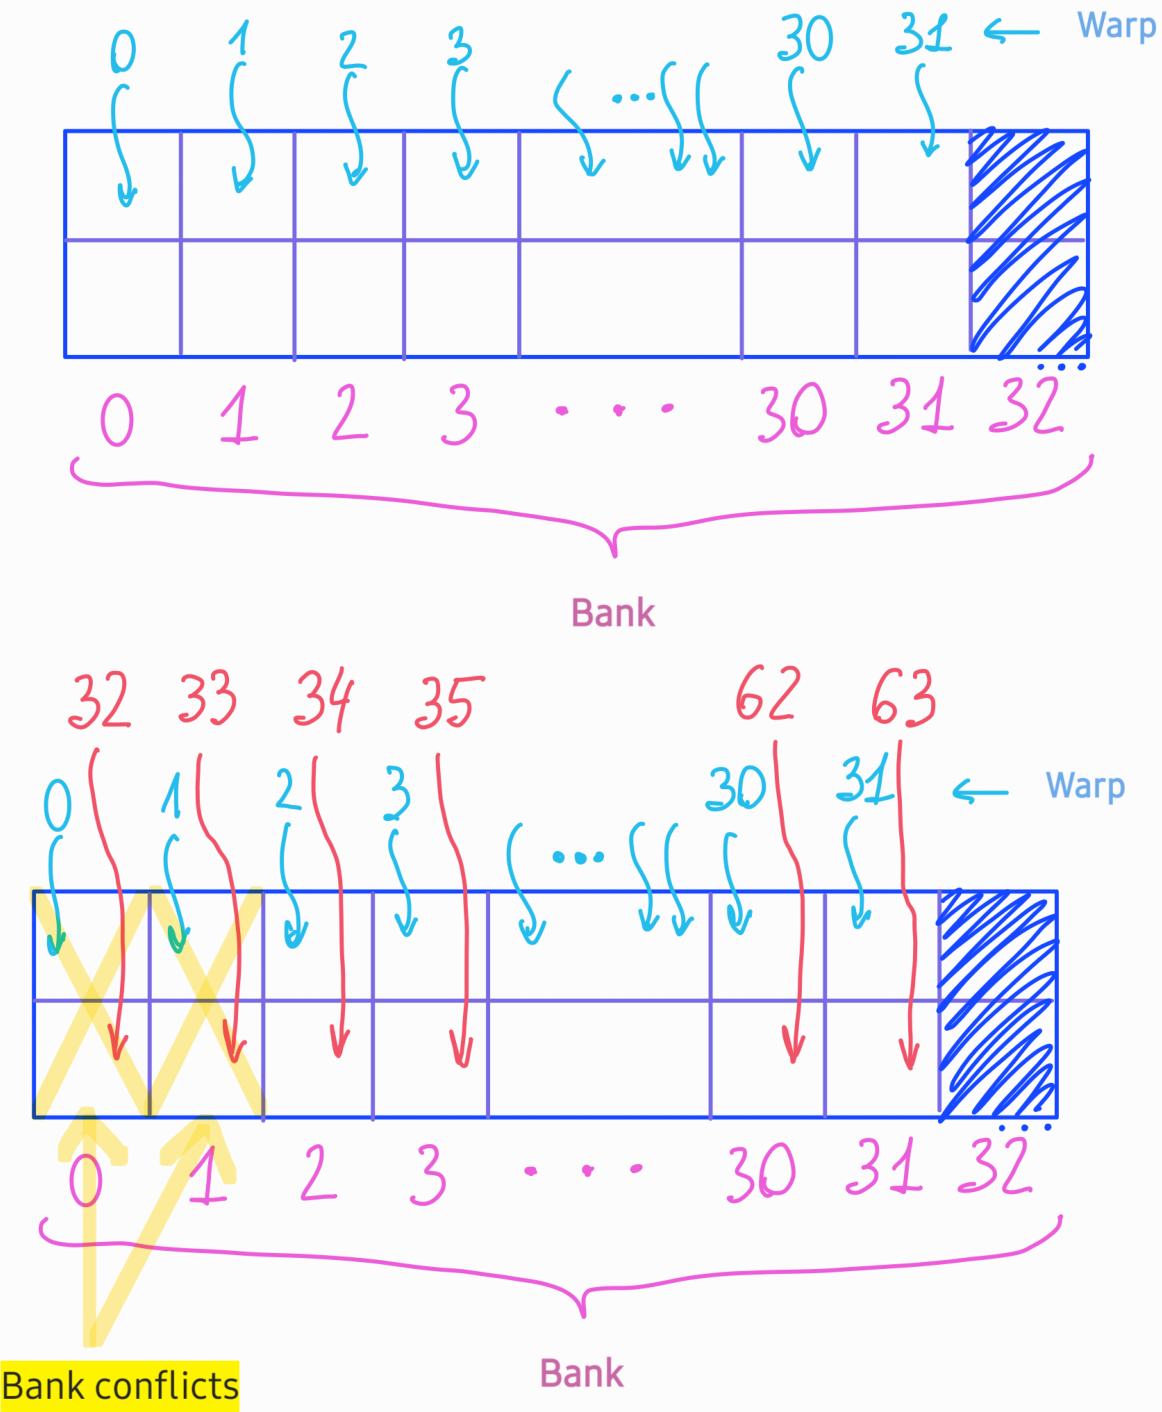
\includegraphics[width=7cm]{pngs/bank_conflict.png} }}
   \qquad
   \subfloat[\centering]{{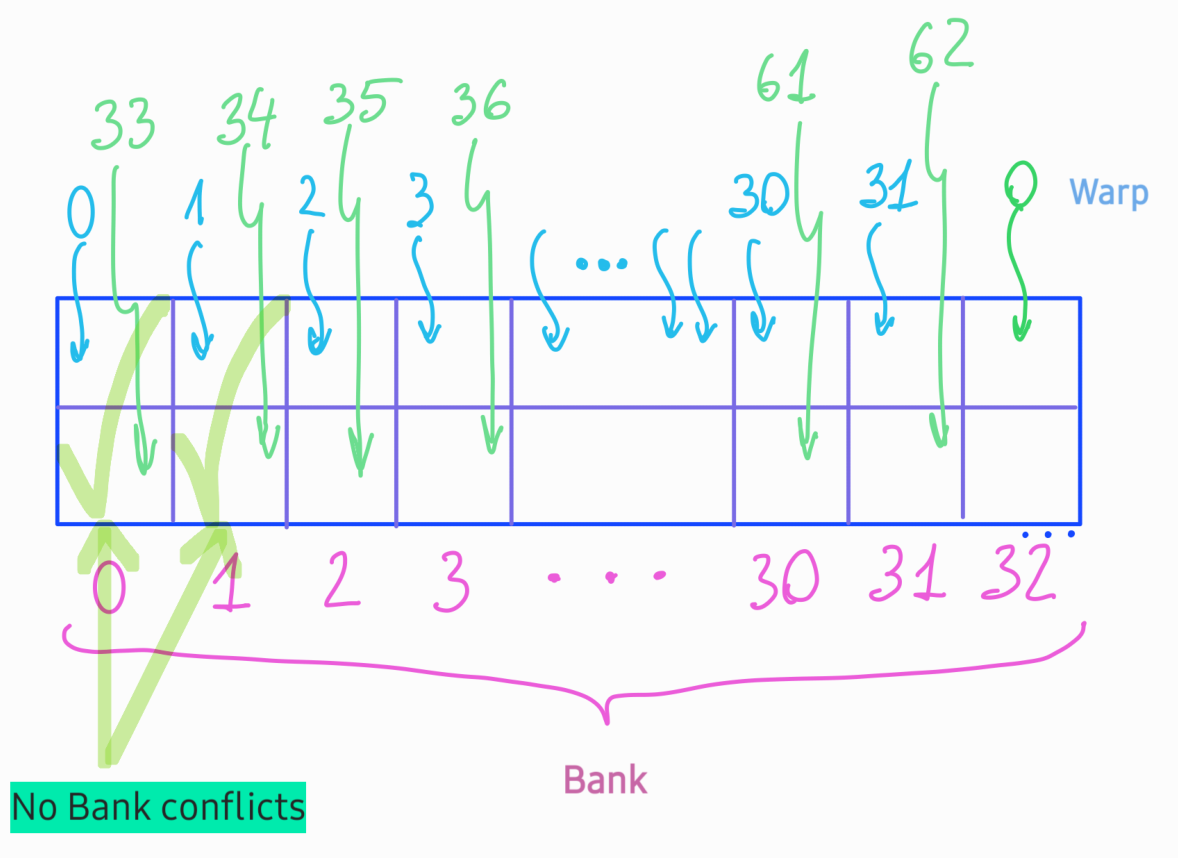
\includegraphics[width=7cm]{pngs/bank_conflict-2.png} }}
   \caption{Bank conflicts}
   \label{fig:bankconflicts2}
\end{figure}

\paragraph{Bank conflicts.} We have practically discussed several applications of the theoretical notions described in the section 
on architecture. How about the bank conflicts? Remember - the warps are chunks of threads (way of scheduling/organizing them). 
The banks are chunks of memory and a way to structure them. Also remember that, ideally, 32 threads, 
organized in one warp, access simultaneously one "column" at a time \autoref{banks}. So if two threads in a warp access simultaneously 
one bank (one column), there is a bank conflict, and the warp will be forced to get split into two execution periods. 
The classical bank conflict is often illustrated by the 2D array initialization in shared memory. 

Once again: suppose we are simply allocating a 1D array (either in global or shared memory) of size 32 bytes. Then one warp is accessing one bank of memory. 
Suppose now we're allocating 64 or 128 bytes of memory, then 2 or 4 warps respectively will access the memory sequentially, i.e. 2 and 4 periods respectively.

So, in order to avoid these bank conflicts in 2D memory (of course, it is always possible to map a 2D array into 1D array, which is much easier to deal with), one should allocate 
\textit{a bit more memory} than required. Take a look at the \autoref{fig:bankconflicts2}: the two first figures (a \& b) show a 1D and 2D array memory access respectively. 
On the LHS, the memory access is a multiple of 32. Therefore, at the same time, more than 2 columns - \textbf{banks}, are accessed by the same warp (multiple of 32). 
In order to get rid of a bank conflict in a 2D memory access, whose size is multiples of 32 (warp's size), we allocate one additional byte to each row (or 4 bytes if it's a float).
To do so, we replace \verb|__shared__ float Mat[BL_SIZE][BL_SIZE]|, with \verb|__shared__ float Mat[BL_SIZE][BL_SIZE+1]|. Indeed, if the addresses are multiples of 32, each warp will 
have to access the same bank/memory address as the previous and the next bank. So, what one can do, is to allocate memory of size 33 rows. Thus, the threads, seeking memory, will 
access different banks(columns).

The author does fully understand and does know that this is a quite subtle aspect, and one needs time to get used 
to these concepts. It is also clear that these things are difficult \sout{or even impossible} to debug and track, once the code is written, and the programmer 
does not have any ideas of where to look for the performance issues. In most cases, 
the \textit{solution} is to simply benchmark the execution of the program, and consequently test the program with different configurations. 

\subsubsection{Other memory addressing}
The main memory, we'll work with is the global and shared memory. However, it would be instructive to have a look at the 
syntax of constant and texture memory allocations. So that, once we come across some of this syntax, we know what is meant 
in this specific piece of code. 

\vspace{-15pt}
\paragraph{Constant memory } is specified with the \verb|__constant__| directive.
Similary as we've done for shared memory with the \verb|__shared__| directive. 
Thus, the constant memory allocation/initialization outside the device code would look something like 
\verb|__constant__ float data[256]|. Now, in the device code, in order to access it, one simply writes \verb|data[i]|.
Now, the next question is how to access this memory from the host code. That is, how to initialize the 
memory from host. To do that, one writes 
 To do that, one writes 
\begin{listing}
\begin{minted}[frame=single, framesep=1mm]{cuda}
//host code
__constant__ float data[256];
cudaMemcpyToSymbol(coeffs, hostData, 256*sizeof(float));
\end{minted}
\caption{Constant memory allocation for device from host. The \textsl{hostData} pointer will be 
the one used in the device code. \cite{talonmies_cudamemcpytosymbol_2013}}
\end{listing}

One can ask ourselves a question on the difference between the mentioned \verb|cudaMemcpyToSymbol()| and \verb|cudaMemcpy()|
functions. The reason, why we can't use the the classical \verb|cudaMemcpy()| function, is because once we declare 
the constant memory using the \verb|__constant__| directive, it has already been explicitly \textit{allocated} and identified as 
constant memory. However, with \verb|cudaMalloc|, we're implicitly assuming, that the memory is global. Therefore, the in order to use 
the \verb|cudaMemcpy()| function, one must first retrieve the address of the constant memory pointer.
For that, we write
\begin{minted}[frame=single, framesep=1mm]{cuda}
//host code
__constant__ float data[256];
float *dcoeffs;
cudaGetSymbolAddress((void **)&dcoeffs, coeffs);
cudaMemcpy(dcoeffs, data, 256*sizeof(float), cudaMemcpyHostToDevice);
\end{minted}
The data can then be used safely from the device.

\vspace{-15}
\paragraph{Texture memory}, as mentioned, will discuss extensively the texture memory. The only 
thing I'll do is to mention, the functions that are associated with the texture memory. The terminology 
for it is similar to the OpenGL's one. That is, vertex buffer objects, vertex array object \cite{noauthor_docsgl_nodate}. Such functions are:

\begin{minted}[frame=single, framesep=1mm]{cuda}
cudaMallocArray() //memory allocation
cudaBindTextureToArray() //memory association with specific texture
\end{minted}

and many others. For more informations : \cite{noauthor_steps3d_nodate}.
%https://stackoverflow.com/questions/16119943/how-and-when-should-i-use-pitched-pointer-with-the-cuda-api

\subsubsection{Memory mapping}
\label{subsub:mem_mapping}
We have discussed multiple kinds of memory - \textbf{Global}, \textbf{Shared}, 
\textbf{thread-local} memories. All of them have different scopes, 
bandwidths, and properties(such as bank access). These memories are classified by their scope, 
not by the way they are allocated and transferred (see \ref{subsection:mem_alloc_model}).

%Until now, we have discussed, that shared memory is invoked with \verb|__shared__| compiler 
%directive. The local memory is thread-local memory, when, for example, we initiate simple memory 
%on stack in a \textbf{kernel}, e.g. \verb|int a = 64| (this \verb|int| a is allocated to each thread's
%register locally). 
%
%The global memory is invoked with \verb|cudaMalloc()| function, called from host. Think of 
%global memory as a \textit{long} transfer between the host and the device. 
%The CUDA API provides, in some ways, to make this process faster. 
%
%
%Note that the following classification is 
%concerning the global memory. \textit{channelling}\footnote{The way the host and the device are 
%communicating with each other, to allocate memory}.
%
%\begin{quote}
%   $\text{HOST}\xRightarrow{\text{owns}}\text{Pageable\& Pinned} \xrightarrow{ALLOCATES}\text{DEVICE}$
%   \label{quote:pinned_pageable}
%\end{quote}

Lets now treat and have a look at different memory allocation types \cite{memory_model}:

\begin{itemize}
   \setlength\itemsep{-0.5em}

   \item \textbf{Pageable data transfer.} When we invoke the \textit{classical} \verb|cudaMalloc()|, 
   we're acessing pageable memory. It is the default behaviour. 
    Under the hood, it is allocated twice - first to pinned memory(see below), 
   then, from the pinned one, to the device global memory. 
      \begin{equation}
        \text{HOST}\xRightarrow{allocates}\text{Pageable} 
        \xRightarrow{} \text{Pinned} \xRightarrow{goes\ to}\text{DEVICE}
      \end{equation}
    One can think of it as the longest path between the host data, 
   and the required device data.
    The syntax for this process is:
    \begin{enumerate}
      \item In order to allocate memory on the host, one uses \verb|malloc()| or \verb|new|.
      \item In order to allocate the memory on the device \verb|cudaMalloc()|.
      \item In order to copy memory from the host to device and vice-versa, one use the \verb|cudaMemcpy()|.
    \end{enumerate}

   \item \textbf{Pinned data transfer} lets us avoid 2-way memory allocation between the host and the device. 
  We are thus skipping one step in the memory allocation pipeline.
   Pinned memory is faster, yet reduces the 
    performance from the host side, as the amount of memory 
    for host processing is reduced.
  The syntax for pinned memory is given by:
    \begin{enumerate}
      \item In order to allocate memory on the host, one uses the \verb|cudaMallocHost()|.
      \item In order to allocate the memory on the device \verb|cudaMalloc()|.
      \item In order to copy memory from the host to device and vice-versa, one use the \verb|cudaMemcpy()|.
    \end{enumerate}

   \item \textbf{Mapped memory}, also called \textit{zero access memory}
     \cite{memory_model}, is pinned memory, which is \textbf{directly} initialized/mapped to the device address. 
    This gives the ability to leverage the device's memory using the host if it is not big enough.
    This also gives a lower memory transfer time. As there is in a way, \textbf{no} memory transfer.
    The syntax for the zero access memory usage is given by:
      \begin{enumerate}
        \item In order to allocate the memory, one uses the \\
          \verb|cudaHostAlloc(void** host_ptr, size_t size, int flags)|, where the flags, e.g. \verb|cudaHostAllocMapped|.
        \item In order to get the communication channel between the host and device, one uses 
          \verb|cudaHostGetDevicePointer()|.
      \end{enumerate}
    You may notice that there is no 2 memory allocations - from the host and device sides. Instead, 
    there is only one memory allocation, and one \textit{pointer sharing}. This emphasizes the \textit{zero mapping}
    fact of the mapped memory.
The flaw of this method is the increase of processing time, as the data is simply mapped, and not copied.

   \item \textbf{Unified memory} is, as its name suggests, memory available both to the host and the device. 
     The biggest advantage of it, is the reduction of the memory allocation pipeline. 
     However, the latency of memory access is highly increased. 
     In order to use and invoke the unified memory, one only uses the \verb|cudaMallocManaged()|. 
     There is no other functions to invoke, as the memory is initialized for both the host and the device.

   \label{mem_alloc}
 \end{itemize}
 Note, that this GPU $\leftrightarrow$ CPU communication is assured via the so-called \textbf{peer access}, 
 which is represented by the \verb|cudaDeviceEnablePeerAccess()| function (see official documentation \cite{center} and \cite{boreskov__nodate}).
  


\subsubsection{Asynchronous memory}
  \label{subsub:async_mem}
  We have seen that both the memory access and memory allocation will affect the program execution time. 
  Therefore when designing a program, one must take into account not only the memory access but also 
  the memory allocation time. 
    The asynchronous memory allocation may reduce the time of program execution, as it is asynchronous. And 
    non-blocking. This concept of asynchronous memory allocation involves the concept of streams discussed 
    further. 
    Therefore the main part of this functionality is discussed in the CUDA streams section \autoref{subsub:async_streams}.
  The asynchronous memory copy is a non-blocking memory copy. The async memory copy is 
  invoked with the \verb|cudaMemcpyAsync()| function. This can be for example used, when one wants to invoke 
  many kernels, with many memory copies. Let's have a look at an abstract example, without going into details, of what is the kernels 
  doing. 
  \begin{listing}
  \begin{minted}[frame=single, framesep=1mm, linenos=true]{cuda}
  for (int i = 0; i < nStreams; ++i){
    int offset = i * streamSize; //offset for memory copy 
    cudaMemcpyAsync(&d_a[offset], &a[offset], streamBytes,\
      cudaMemcpyHostToDevice, stream[i]);
    kernel<<<streamSize/blockSize, blockSize, 0,\
      stream[i]>>>(d_a, offset);
    cudaMemcpyAsync(&a[offset], &d_a[offset], streamBytes,\
      cudaMemcpyDeviceToHost, stream[i]);
  }
  \end{minted}
  \caption{The code snippet \cite{async_memcpy} is giving an example of how to use the asynchronous memory copy. 
Thanks to the streams combination with the async memory copy, the only synchronization that is happening is the memory copy and kernel execution, inside 
a separate stream. That is, if no streams are specified, every iteration is will wait for the previous one to finish. For details, see \autoref{sec:streams}.}
\end{listing}

